\documentclass{article}
\usepackage[utf8]{inputenc}
\usepackage[english, spanish]{babel}
\usepackage[dvips]{graphics}
\usepackage{amsmath}
\usepackage{amssymb}
\usepackage{fullpage}
\usepackage{epsfig}
\usepackage{multicol}
\usepackage{listings}
\usepackage{wasysym}

\usepackage[usenames,dvipsnames]{xcolor} 
\usepackage{hyperref} 
\definecolor{linkcolour}{rgb}{0,0.2,0.6} 
\hypersetup{colorlinks,breaklinks,urlcolor=linkcolour,linkcolor=linkcolour} 
\newcommand{\parallelsum}{\mathbin{\!/\mkern-5mu/\!}}



\parindent 0pt
\parskip 0pt

\begin{document}


\includegraphics[width=4.6cm, height=1.7cm]{logor.png}
\vspace*{-1.55cm}

\hspace*{1.4 cm}
 \hspace*{2.9 cm}
 {\footnotesize
 \begin{tabular}{l}
  \sc IM Trust - Credicorp Capital\\
  \sc Administradora General de Fondos \\
  \sc Mesa de Gestión de Inversiones  \\
  \sc Diego Steinsapir  \\
  \vspace{15\baselineskip}\mbox{}
  \vspace{-3mm}\mbox{}
 \end{tabular}
}

 \bigskip

\vspace*{5mm}
\begin{center}
{\today} \\
\vspace{3mm}
{\Large\bf Generación de Excel para Reporte de Seguimiento} \\
\vspace{2mm}
\end{center}
%%%%%%%%%%%%%%%%%%%%%%%%%%%%%%%%%%%%MANENER FIJO ARRIBA%%%%%%%%%%%%%%%%%%%%%%%%%%%%%%%%%%%%%%%%%%%%%%%%%%%%%%%%%%%%%%%%%%%%%%%%%%%%%%%%%%%%%%%%%%%%
\section{Introducción}


Para cada cartera, es necesario periodicamente producir un Reporte de Seguimiento en el cual se especifique la evolución de su rendimiento. De esta manera, el Reporte de Seguimiento muestra los cambios en la rentabilidad de la cartera y su composición para un periodo, además de los movimientos generados y junto con más información relevante. En el presente documento se detallan las principales características, usos y explicaciones del programa y sus principales métodos creado para la generación automática del archivo Excel utilizado para los Reportes de Seguimiento.

\section{Generación de Reporte de Seguimiento}

\subsection{Materiales}

Para la generación automática del archivo Excel con la información necesaria para el Reporte de Seguimiento, es necesario contar con dos archivos:

\begin{itemize}
\item generador.exe: Archivo ejecutable encargado de recopilar y analizar datos necesarios para transformarlos en información utilizable en el Reporte de Seguimiento
\item seguimiento.xlsm: Archivo de Excel preformateado sobre el cual seguimiento.exe lee paramétros iniciales y luego edita con la información final para Reporte.
\end{itemize}  

\subsection{Modo de Uso}
Para generar el Excel para el Reporte de Seguimiento de manera automática, se deben seguir los pasos a continuación:

\begin{enumerate}
\item Abrir seguimiento.xlsm y en la hoja "Control" escribir el código del fondo a evaluar y las fechas entre las cuales se desea evaluar. Las fechas deben ir en formato 'AAAA-MM-DD'. NO editar nada más.Guardar y cerrar archivo

\begin{center}
\begin{figure}[h!]
\graphicspath{ {./} }
\centerline{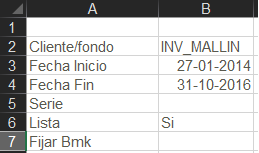
\includegraphics[scale=0.8]{Control}}
\caption{Grafico 1 Ejemplo de edición de hoja Control}
\end{figure}
\end{center}

\item Ejecutar generador.exe. Elegir archivo seguimiento.xlsm editado cuando aparezca el diálogo pidiéndolo. Esperar a que se termine de ejecutar cuidando no interactuar con el Excel que se abra.

\end{enumerate}

\subsection{Output}
Tras finalizar la ejecución, el programa generará un archivo Excel con todas las tablas y gráficos en formatos correctos listos para su utilización en el Reporte. Dicho programa se generará en una carpeta a eleccin por el usuario y tendrá el nombre  {CodigoFondo\_FechaCreación.xlsm}

\section{Detalle de Archivos}
A continuación, se describirá de manera más específica cada archivo utilizado.

\subsection{seguimiento.xlsm}
\subsubsection{Estructura}
El archivo seguimiento.xlsm corresponde a un libro de Excel con Macros habilitados. En el se poblarán los datos relevantes para el Reporte de Seguimiento y se generarán las tablas y gráficos necesarios. Se entrega con una estructura establecida y con el diseño de tablas y gráficos corporativo incluido. 

Se estructuran las hojas de la siguiente manera:
\begin{itemize}
\item Control: En esta hoja se deben ingresar los parámetros a leer para la generación del resto del archivo Excel
\item Datos: Aquí se imprimirán los valores cuota del portafolio, junto con retornos mensuales y anuales para cada uno. Los retornos se calculan con el programa generador.exe. 
\item SEGUIMIENTO: Aquí se imprimirán las tablas y gráficos relevantes para el Reporte de Gestión con su formato y diseño correcto. Es importante destacar que estos elementos se generan desde el Excel mismo. Vale decir, el archivo seguimiento.xlsm viene con los gráficos creados, pero sin los datos neceasrios. Esto se hace de esta manera para permitir la edición de datos si es necesario, además de dar una mayor visibilidad del origen de los datos mismos. Finalmente, ello permite asegurar de antes (y editar a posteriori) el diseño utilizado en cada uno.
\item CarteraCompleta: Se imprimen todos los instrumentos incluidos en el portafolio junto con todas sus clasificaciones de todo tipo.
\item Cartera-Neutral: Se imprime el detalle de la Cartera-Neutral \footnote{29-12-2016: Aun debe hacerse, pero hoja está creada}
\item CarteraRFL, CarteraRVL, CarteraRFI, CarteraRVI: Se imprimen los instrumentos de cada clase de activo mayor (RFL, RVL, RFI, RVI), separados por subclase
\item ResumenCartera: Se imprimen las tablas de las principales descomposiciones de la cartera completa en monto y pocentaje. Por ejemplo:
\begin{table}[h!]
\centering
\begin{tabular}{cll}
Moneda & Monto  & Porcentaje \\
\$      & 10.000 & 0,25      \\
UF     & 30.000 & 0,75      
\end{tabular}
\end{table}

\item ResumenCarteraLabel: Igual a hoja "ResumenCartera", pero quita columnas de montos y agrega etiquetas a entradas para generar gráficos con formato correcto

\item ResumenCarteraRF: Igual a ResumenCartera, pero creado de forma específica para la Renta Fija Local
\item ResumenCarteraRFLabel: Equivalente a ResumenCarteraLabel pero para Renta Fija
\item Información Cartera/Argupar Información Cartera: Botón para esconder/mostrar pestañas de desgloses de cartera para hacer Excel más ordenado
\item Evolucion: En esta hoja estarán disponibles los gráficos de la evolución de la cartera según su composición por clase de activo, moneda y mercado
\item DataEvolucion: Aquí se encontrará en forma de tabla la información necesaria para generar los gráficos de la evolución de la cartera en la hoja "Evolucion"

\end{itemize}
\subsubsection{Avance futuro}
Se debe agregar en el futuro una hoja en que se detallen los movimientos de la cartera, como aportes y rescates y pagos de dividendos

\subsection{generador.exe}
En esta sección se explican los métodos más importantes y complejos del código junto con el flujo completo y desiciones de diseño y tecnologías. 
\subsubsection{Tecnología}
El programa fue escrito con Python 3.5.2 y está versionado con Git en el repositorio 
\begin{center}
\texttt{mesagi/Proyectos/generador\_presentacion\_gestionactivos}
\end{center}
\subsubsection{Diseño}
Para mayor mantenibilidad y facilidad de lectura, el código se ha separado en distintos archivos. Un archivo llamado generador.py contiene el flujo principal del program (método "main"), otro llamado seguimiento.py es la librería con los métodos utilizados por generador.py, y el resto de los archivos corresponde a las consultas SQL necesarias para el programa.

Dentro del código se prioriza no usar variables globales (no así, constantes globales) para faciilitar el entendimiento del código. Al principio de cada archivo se especifican las constantes utilizadas (nombres de hojas, parametros y entradas en bases de datos). Si por alguna razón alguno de estos valores se cambiará, basta cambiar los valores al principio del archivo para volver al funcionamiento normal. 
\subsubsection{Principales Métodos}
\begin{itemize}
\item calculateReturns(data, index): Calcula los retornos mensuales y anuales de un portafolio y su benchmark a partir de los valores diarios.
\begin{lstlisting}
def calculateReturns(data, index):  # 1 para fondo, 2 para benchmark
    currentDayForMonth = data[0] # Init values
    currentDayForYear = data[0]
    monthlyReturns = []
    yearlyReturns = []

    # NOTE Datos ya vienen ordenados en forma desc
    for day in data:
      if currentDayForMonth[0].month != day[0].month:
          currentMonthReturn = currentDayForMonth[index] /
            			day[index] - 1
          currentMonthBenchmarkReturn = currentDayForMonth[index + 1] /
            				day[index + 1] - 1
          monthlyReturns.append([str(currentDayForMonth[0].month)
                                   + "/" + str(currentDayForMonth[0].year),
                                   currentMonthReturn,
                                   currentMonthBenchmarkReturn])
          currentDayForMonth = day
          if currentDayForYear[0].year != day[0].year:
              currentYearReturn = currentDayForYear[index] / day[index] - 1
              currentYearBenchmarkReturn = currentDayForYear[index + 1] /
              					day[index + 1] - 1
              yearlyReturns.append([currentDayForYear[0].year,
                                    currentYearReturn,
                                    currentYearBenchmarkReturn])
              currentDayForYear = day
\end{lstlisting}

En esta primera parte, se aprovecha que los valores de la cartera y el benchmark vienen ya ordenados por fecha. Luego, se toma el primer valor de estos datos y se itera sobre las demás entradas hasta deetectar un cambio de mes. Una vez que se identifica un cambio de mes, se divide el valor original por el primero del mes nuevo (dia 31 o 30 del mes anterior) para obtener la rentabilidad de ese mes. Luego, se actualiza el valor contra el cual comparar y se hace lo mismo para el siguiente mes hasta terminar los datos. Cuando se detecta un cambio de mes se verifica también un cambio de año para obtener el retorno anual con la misma lógica. 

Lo anterior deja afuera la rentabilidad del último mes y año (más lejano al día de hoy). Para incluirlo, el método termina de la siguiente manera:

\begin{lstlisting}
    # Incluir ultimo mes
    last = data[len(data) - 1]
    if currentDayForMonth[0].month == last[0].month:
      lastMonthReturn = currentDayForMonth[index] / last[index] - 1
      lastMonthBenchmarkReturn = currentDayForMonth[index + 1] /
      				last[index + 1] - 1
      monthlyReturns.append([str(last[0].month) + "/" + str(last[0].year),
                               lastMonthReturn, lastMonthBenchmarkReturn])

    # Incluir ultimo anio
    if currentDayForYear[0].year == last[0].year:
      lastYearReturn = currentDayForYear[index] / last[index] - 1
      lastYearBenchmarkReturn = currentDayForYear[index + 1] /
      				last[index + 1] - 1
      yearlyReturns.append([last[0].year,
      			lastYearReturn,
      			lastYearBenchmarkReturn])

    return (monthlyReturns, yearlyReturns)
\end{lstlisting}

\item subclassify(portfolio): Se utiliza para entregar a cada instrumento en el portafolio las subcategorías que son relevantes para el Reporte de Seguimiento pero que no están explícitas en las bases de datos

\begin{lstlisting}
def subclassify(portfolio):
    # Indices de columnas
    instrumentTypeIndex = portfolio[0].index(TIPOINSTRUMENTO)
    zoneIndex = portfolio[0].index(ZONA)
    durationIndex = portfolio[0].index(DURATIONHEADER)
    riskIndex = portfolio[0].index(CLASIFICACIONRIESGO)
    currencyIndex = portfolio[0].index(MONEDA)
    incomeTypeIndex = portfolio[0].index(RENTA)
    amountIndex = portfolio[0].index(MONTO)
\end{lstlisting}

Primero se busca en qué indice dentro del arreglo está cada título de columna de la tabla. Cabe notar que portafolio es una tupla de dos datos, en que el primer datos corresponde a un arreglo de títulos y el segundo a los datos mismos. Esto deja a portfolio de la forma portfolio = <Titulos, Datos>. También es importante destacar que las constantes que se están dando como parámetro en cada caso corresponde a los títulos actuales en la base de datos (por ejemplo, MONEDA = "Moneda"), que en caso de cambiar deben modificarse también en este archivo al principio. Esta lógica se utiliza en más métodos.

\begin{lstlisting}
i = 0
totalAmount = sum(row[amountIndex] for row in portfolio[1])
for instr in portfolio[1]:
        # Porcentaje. NOTE: Float necesario por bug xlwing
        percentage = float(instr[amountIndex] / totalAmount)
        # Zona
        zone = instr[zoneIndex]
        # Corto_Largo
        short_long = 'Corto' if instr[durationIndex] <= DURATION else 'Largo'
        # Moneda
        currency = instr[currencyIndex]
\end{lstlisting}

\begin{center} 
\dots
\end{center}

Esto se continua para varias mas categorías. Se agrega ademas lo siguiente para poder detectar los fondos que serian subclasificados como liquidez y como mal clasificados. Aquellos mlas clasificados se les entrega la asset\_class y subclase virtual 'NC' (No Clasificado).
\begin{lstlisting}
        # Asset Class y Subclass, tomando en consideracion que podrian ser liquidez
        if "CFM8401" in instr[instrumentCodeIndex] or 
          instr[emmitterIndex] in ["LIQUIDEZ", "CAJA"]:
            assetClass = "Liquidez " + instr[currencyIndex]
            subclass = "Liquidez " + instr[currencyIndex]
        else:
            assetClass = getClass(incomeType, zone, country)
            subclass = getSubclass(zone, currency, risk,
                      instrumentType, short_long, incomeType, country)

        # Clasificacion Falsa para detectar incorrectos
        if detectWrongClassification(instr):
            assetClass = "NC"
            subclass = "NC"
\end{lstlisting}

Luego, se agrega en el arreglo de datos todas las nuevas categorías:
\begin{lstlisting}
        # Extender todo
        instr += (percentage,
                  short_long,
                  risk_duration_currency,
                  risk_duration,
                  duration_currency,
                  instrumentType_Currency,
                  instrumentType_duration,
                  assetClass,
                  subclass)

        portfolio[1][i] = instr
        i += 1
\end{lstlisting}

Con el loop finalizado, se agregan los nuevos títulos y se retorna portfolio. El método entonces solo ha extendido nuevas categorías a los datos recopilados desde la base de datos:
\begin{lstlisting}
    # Agregar nuevos titulos
    portfolio[0].extend(["Porcentaje",
                         CORTOLARGO,
                         RIESGODURACIONMONEDA,
                         RIESGODURACION,
                         DURACIONMONEDA,
                         TIPOINSTRUMENTOMONEDA,
                         TIPOINSTRUMENTOLARGO,
                         ASSETCLASS,
                         SUBCLASS])

    return portfolio
\end{lstlisting}

\item assetClassBreakdown(headers, subportfolio): Divide un portafolio por subclases y lo devuelve como un \href{https://en.wikipedia.org/wiki/Associative_array}{diccionario} con cada subclase como llave y los instrumentos de esa subclase en un arreglo como valor de la llave. 
La siguiente linea se encarga de obtener un arreglo con todas las llaves del diccionario de forma única a partir de las subclases observadas en el subportafolio:
\begin{lstlisting}
subclasses = set(np.column_stack(subportfolio)[subclassIndex])
\end{lstlisting}
Después de esto, se genera un diccionario y se itera para agregarlos al arreglo de instrumentos correspondiente a su subclase en la llave del diccionario.


\item totalPerType(typeIndex, amountIndex, matrix): Se utiliza para la generación de los resumenes de cartera y devuelve el monto y porcentaje invertido en los instrumentos según alguna categoría. Se le entrega un indice de la columna de la cual se quiere hacer resumen en typeIndex y el índice en el que se encuentra el monto invertido en ese instrumento, junto con la matriz de datos. Por ejemplo, si se tiene una matriz de datos en que las columnas siguen el orden <Moneda, TipoInstrumento, Emisor, Riesgo, Monto, Duracion> y se quiere hacer un resumen sobre los Emisores, el método se llama como:
\begin{lstlisting}
totales = totalPerType(2, 4, data)
>>> totales = [
>>> Emisor1: [15.000, 0,2], 
>>> Emisor2: [30.000, 0,4], 
>>> Emisor3: [30.000, 0,4]]
\end{lstlisting}

\item printPortfolioSummary(workbook, sheet, portfolio, RFL): Utiliza el método totalPerType para imprimir en Excel todos los resumenes que resultan interesantes. Se agrega un valor booleano RFL para distinguir las categorías que se quieren resumir en caso que se esté evaluando la subcartera de Renta Fija Local

\item printLabeledSummary(workbook, sheet, totals): Imprime lo mismo que el método anterior, pero con la diferencia que agrega etiquetas con formato listo para generar gráficos en Excel.

\item printPortfolioCompositionPies(workbook, sheet, datasourceSheet, piesAmount, lastIndex): Se utiliza para generar los gráficos de torta. Es necesario destacar que en el Excel hay otros gráficos que se arman directamente desde el mismo archivo, pero los gráficos de torta no se comportaban muy bien si se dejaban prearmados con los datos listos. Para solucionar esto, se crean en el archivo Excel gráficos con el diseño correcto, \underline{pero sin datos}. Luego, el programa lee cada uno de estos objetos y los llena con los datos correctos.
El método funciona primero leyendo los objetos "charts" de una determinada hoja y luego asignándole su conjunto de datos.

\item getStatistics(data): Obtiene estadísticas importantes para el set de datos de valores cuota de portafolio y benchmark entregados. Cada dato de la matriz es de la forma [Fecha, Retorno Portafolio, Retorno Benchmark]. Los indicadores estadísticos que entrega son:
\begin{itemize}
\item Alpha
\item Beta
\item Tracking Error
\item R cuadrado
\item Volatilidad Portafolio
\item Volatilidad Benchmark
\end{itemize}
La obtención de todas las estadísticas - a excepción del Tracking Error - se basa en el código encontrado en \href{http://gouthamanbalaraman.com/blog/calculating-stock-beta.html}{http://gouthamanbalaraman.com/blog/calculating-stock-beta.html}, donde además hay una explicación de cada una. El tracking error por su parte, se calculó como la varianza del vector de alpha's, con alpha calculado como la diferencia entre los retornos de la cartera y el benchmark. Vale decir:
\begin{center}
Tracking Error = var \begin{pmatrix}
\alpha_{1} \\ \alpha_{2} \\ \vdots \\ \alpha_{N}
\end{pmatrix}
= var \begin{pmatrix}
R_{1} - R_{1}^{b} \\ R_{2} - R_{2}^{b} \\ \vdots \\ R_{N} - R_{N}^{b}
\end{pmatrix} 
\end{center}

\item extractByTimedelta: De un conjunto de datos, retorna aquellos que se encuentren dentro de una diferencia (delta) de fechas determinada. 

\item binarySearchFirstEntry: Implementación del algoritmo de \href{https://en.wikipedia.org/wiki/Binary_search_algorithm}{búsqueda binaria} ($\Theta$(log (n)), O(n)) para encontrar la fecha del primer dato disponible dentro del rango de un rango de fechas determinado. Por ejemplo, si se pregunta por datos de una cartera entre 05-11-2010 y 21-05-2016 y el primer dato corresponde al 12-09-2014, este método retorna 12-09-2014. 

\underline{Nota}: Se optó por esto debido a la complejidad de la base de datos. Buscar según MIN(fecha) en la tabla ZHIS\_CARTERAS\_MAIN demora mucho, mientras la consulta usada para este método era mucho menos costosa y puede usarse varias veces debido a esto.

\item getLastPortfolioOfMonth: Se utiliza para encontrar la composición del último portafolio registrado de un mes. Se le entrega una fecha correspondiente al último día de un mes (ej: 31-03-2015) y la consulta que devuelve los instrumentos encotnrados en el portafolio a esa fecha. Luego, va iterando hacia atras hasta encontrar un día del cual se cuenten con registros.

\item portfolioCompositionTimeSeries: Utilizado para encontrar la evolución de la cartera en el tiempo en tériminos de su composición por clase de activo, moneda y mercado en el que se invierte. Primero utiliza binarySearchFirstEntry para encontrar la fecha del primer registro. Con este dato, encuentra todas las fechas desde esta fecha hasta la fecha consultada y las remuestrea para tener solamente el último día de cada mes. Tras esto, las deja en formato correcto. To ello se hace en las siguientes líneas:
\begin{lstlisting}
for i in range(1, delta.days + 1):
    dates.append(minDate + td(days=i))

samples = pd.DataFrame(dates, columns=["Date"])
samples = samples.set_index("Date")
samples = samples.resample('M').last()
samples.reset_index(drop=False, inplace=True)
samples.drop(0, inplace=True)
\end{lstlisting}
\item printPortfolioEvolution: Este método se utiliza para poder imprimir la evolución de la cartera en términos de clases de activo, moneda y mercado de inversión. Se utiliza de la mano de portfolioCompositionTimeSeries. En particular, el método comienza por dejar la información de la evolución de la cartera en forma matricial para lograr un manejo de los datos más sencillo. Luego, lee los objectos 'Charts' ya creado en el Excel en la página 'evolucion' y les  asigna su dataset para que se cree el gráfico correspondiente. Es equivalente a la creación de los gráficos de pies.

\item main: El programa principal es bastante directo. Primero genera una conexión a la base de datos con las constantes declaradas al principio del programa. Luego hace una consulta a la base de datos por los valores cuota diarios entre las fechas especificadas para el portafolio y su benchmark, desde lo cual calcula los retornos. Luego consulta por los instrumentos que componen el portafolio y los imprime primero de manera completa, después de manera desglosada, y finalmente de manera resumida. 

\item resource\_path: Sirve para leer archivos tanto en modo de desarrollo (corriendo el código desde la terminal sin un ejecutable) y en modo de producción (desde el ejecutable compilado). Este método es necesario para poder distribuir el archivo ejectuable sin necesidad de además distribuir las queries a la base de datos. El uso de MEIPASS, se explica en la documentación de PyInstaller en \href{https://pythonhosted.org/PyInstaller/runtime-information.html}{este link}


\end{itemize}

\subsubsection{Compilación}
La compilación de generador.exe se hizo utilizando la librería \href{http://www.pyinstaller.org/}{PyInstaller} Versión 3.2, con un equipo con Windows 10 instalado (64 bits) y Python 3.5.2, además de todas las librerías neceasrias para el programa. La compilación puede, en teoría, lograrse con otras librerías creadas con este fin (Py2Exe, cx\_Freeze, etc.), sin embargo en este caso solo se logró con PyInstaller. Para el detalle de la compilación paso por paso, referirse al documento Manual de Compilación 

\subsubsection{Posibles extensiones}
\begin{itemize}
\item Los errores debiesen manejarse de mejor manera, mostrando los errores nativos de Python además del mensaje de error que hay actualmente.
\end{itemize}


\section{Puntos de Falla}
\begin{itemize}
\item Existe un bug que ocurre a veces al finalizar la ejecución, en que Excel se congela o no corre bien. Basta cerrar todas sus instancias y volver a correr Excel. Se puede arreglar si se cambia la línea 
\begin{lstlisting}
workbook = Mesa.openWorkbook(filePath, False, False)
\end{lstlisting}
por 
\begin{lstlisting}
workbook = Mesa.openWorkbook(filePath, True, True)
\end{lstlisting}
Sin embargo, hace al programa mucho más lento. 
\textbf{\underline{RECOMENDACIÓN}}: Guardar todo antes de correr el programa. 
\item A veces el programa se congela si hay alguna celda seleccionada y su formula en edición. Deseleccionar y debiese correr sin problemas
\end{itemize}

\end{document}


